\documentclass[acmsmall, screen, nonacm, 9pt, a4paper,top=2cm,bottom=2cm,left=1cm,right=1cm, marginparwidth=1cm]{acmart}
\usepackage[english]{babel}

% Replace `letterpaper' with `a4paper' for UK/EU standard size
% \usepackage[a4paper,top=2cm,bottom=2cm,left=1cm,right=1cm,marginparwidth=1cm]{geometry}

% Useful packages
% \usepackage{amsmath}
% \usepackage{graphicx}
\usepackage{float}  
\usepackage{pdfpages}


% remove author addresses
\makeatletter
\let\@authorsaddresses\@empty
\makeatother


\title{BeFeel}
\author{Philip Mortimer}
\author{five other students}

\begin{document}
\maketitle
\pagestyle{plain}


\section{Motivation}
Mental health issues are rising amongst university students \cite{Storrie2010AProblem}, with 17\% experiencing psychiatric disorders \cite{Macaskill2013TheKingdom}. Despite this, the vast majority of students do not seek treatment \cite{Macaskill2013TheKingdom,Blanco2008MentalPeers}, primarily due to the stigma associated with mental disorders \cite{MichaelN.Sharpe2004TheEducation}. Distressed individuals typically tend to be unaware of how to seek help and often lack effective coping mechanisms to manage their wellbeing \cite{Rosenthal2008MentalStudents}.

Artificial Intelligence (AI) powered chatbots have shown promise in supporting people with mental health issues by allowing them instantaneous and anonymous access to therapeutic conversations\cite{Grove2021Co-developingPeople}. Whilst there are limitations, recent advances in conversational AI have demonstrated that chatbots are capable of exhibiting human-like intelligence in conversation \cite{Bubeck2023SparksGPT-4}, which makes them promising candidates for providing effective mental health support \cite{Pham2022ArtificialPsychiatry}.

The ubiquity of smartphones amongst students \cite{OfcomSmartphoneStatista} presents an opportunity to leverage technology to monitor and improve mental wellbeing without necessarily requiring specialist supervision. Smartphone applications have shown to be effective at continuous mental health monitoring through the tracking of factors such as sleep quality, exercise regime and social interactions \cite{Wang2014StudentLife,Wang2022First-GenLens}. However, such applications are currently severely limited by their inability to act on data to provide support for users.

\emph{BeFeel} aims to use continuous mental health monitoring to produce achievable goals for students to improve their mental wellbeing. A chatbot will be utilised to receive regular user wellness feedback and provide conversational support. Additionally, struggling users will be given a one-click button that allows them to reach out to university wellbeing services, hopefully alleviating the difficulties associated with obtaining support. Proposed is a unique solution that hopes to enhance the mental wellness of university students through its innovative approach.

\section{Idea}
\emph{BeFeel} is a smartphone application designed to help university students achieve sustained mental wellbeing. \emph{BeFeel} tracks activity levels, sleep habits and screen time amongst other factors to continuously monitor the emotional state of users. The full list of attributes tracked is described in \emph{Figure 1.5}, with participants being able to select the information that they feel comfortable sharing. This informed consent is important \cite{MozillaOurIncluded} as our HCI process and ethical analysis uncovered significant concerns about data collection.

Users primarily interact with the app through an AI chatbot, personified by a customisable avatar; the avatar sends the user daily text messages to check in on their mood and provide them with the support they require. Use of an AI persona targets the stigma that some students feel when discussing their issues with medical experts \cite{MichaelN.Sharpe2004TheEducation} and alleviates the challenges young people face when seeking mental health assistance \cite{Biddle2004FactorsSurvey.}. Research suggests that AI chatbots offer several benefits over professional support as they are available at all times and have greater capacity to tailor to individual needs, whilst still maintaining interaction authenticity \cite{Brandtzaeg2022MyFriendship}. Auto-generated responses are suggested to the user, facilitating fast communication, and encouraging sustained engagement with the chatbot.

Tracked user data is combined with conversation history to assess the mental state of users and generate goals that can be enacted to improve mental wellbeing. These goals are designed to be achievable and are a combination of short and medium-term goals. An example goal may be to go for a 30 minute walk in a day, particularly if sensor data indicates a sedentary lifestyle. A summary of these goals is presented on the home screen for ease of access. Our chatbot will send follow up messages to remind users of their goals and will respond to users achieving or falling short of their targets appropriately. This adaptive approach allows for natural habit building, hopefully leading to a lasting state of mental wellness. A widget displaying the goals that the user should currently be working towards is also included. This provision of focused information should help users have a clear idea \cite{ThereseFessendenAesthetic8} of exactly what they can do to improve their emotional state.

Continuous mood tracking enables \emph{BeFeel} to detect when users should reach out for professional support. When this occurs, users are given a one-click button which allows them to contact university wellbeing services, completing the relevant forms on the user’s behalf. This ease of access is important as a common barrier to obtaining support is difficulty locating and filling out relevant care-preceding documents \cite{Rosenthal2008MentalStudents}. It is important to stress that \emph{BeFeel} is not intended to act as a substitute for professional care, although it can be effectively deployed in conjunction with treatment. If \emph{BeFeel} detects that users are distressed, it prompts them to call a suicide prevention hotline. In addition to this, \emph{BeFeel} also provides a set of external mental health websites and contacts to encourage engagement with a wide range of effective wellbeing techniques. These steps have been taken to safeguard our vulnerable user group and increase the likelihood of a long-term positive outcome.

\emph{BeFeel} will enable university students to lead happier and healthier lives through its adaptive goal setting, conversational support and one-click outreach facility.


\section{Storyboard and Prototypes}
\begin{figure}[H]
    \centering
    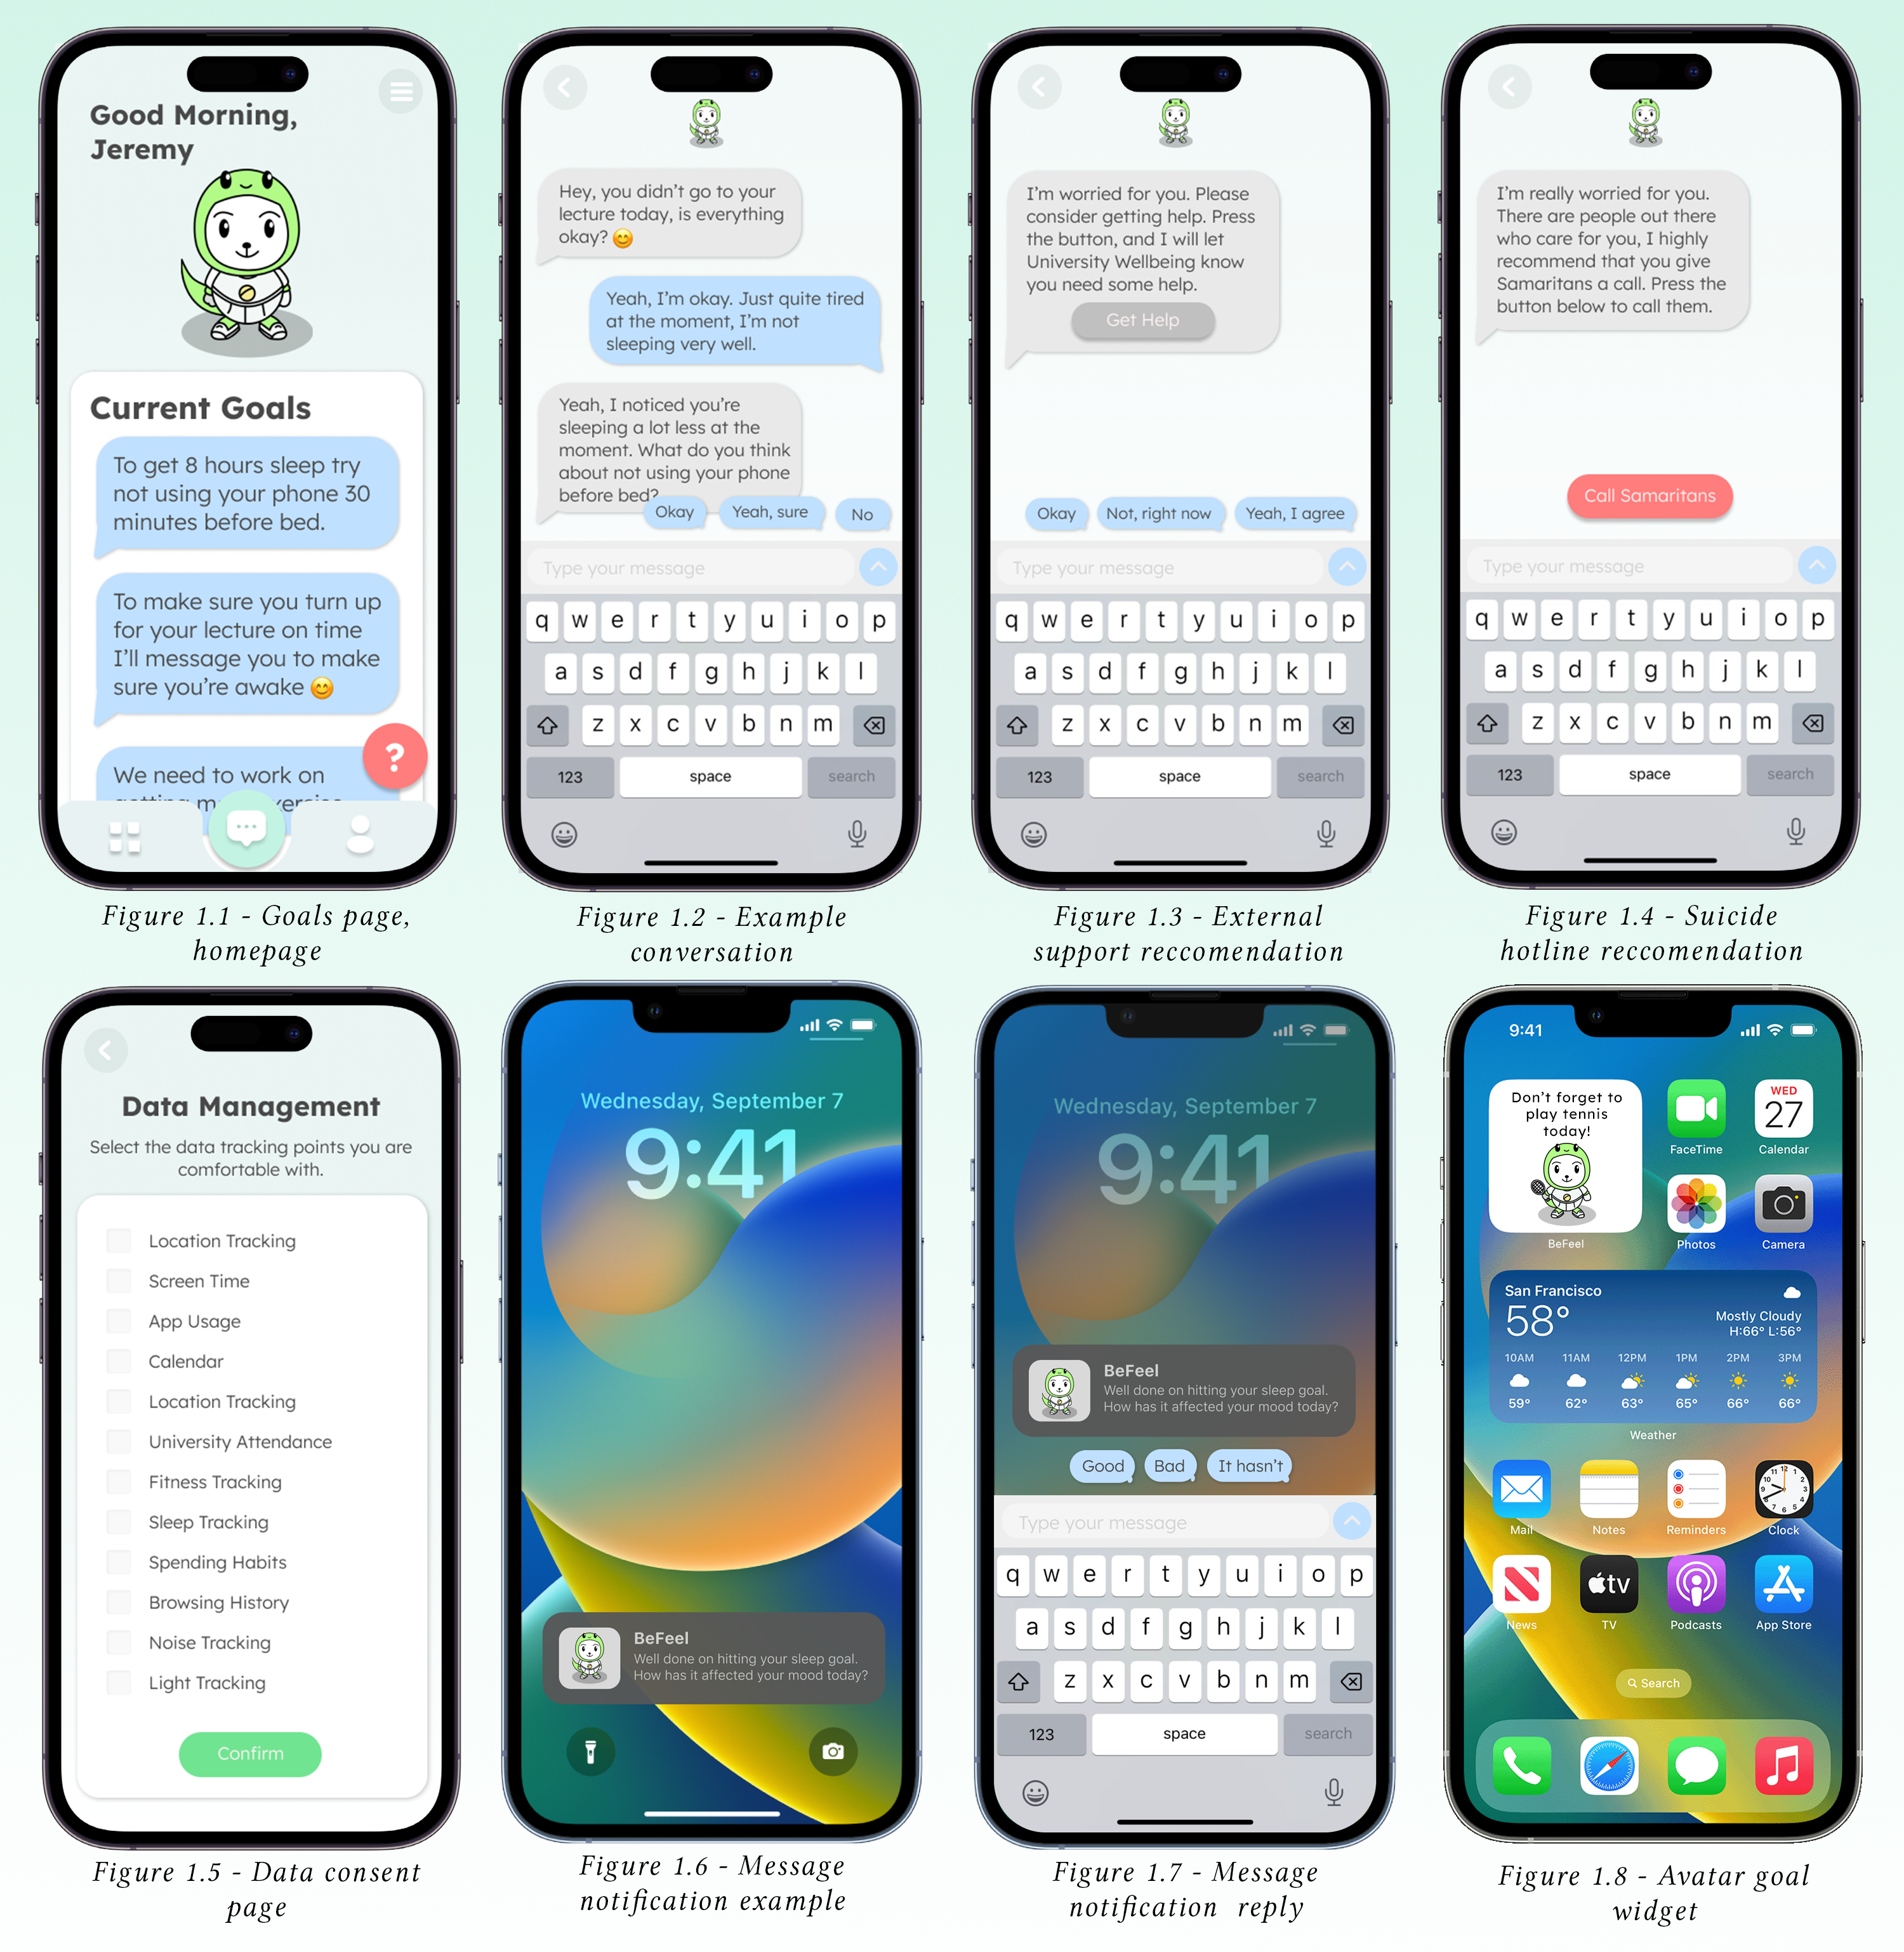
\includegraphics[width=\linewidth]{beFeel.png}
    \caption{Schematics of BeFeel app}
    \label{fig:beFeel}
    
\end{figure}

\begin{figure}[H]
    \centering
    
\includegraphics[width=0.95\linewidth]{storyboard.png}
    \caption{Storyboard depicting a user's journey (Images generated with MidJourney)}
    \label{fig:storyboard-main}
\end{figure}



\section{Background and Related Work}
Many studies exist that attempt to quantify and record the mental state of students, most notably \emph{StudentLife}. In this study of 48 students at Dartmouth College, the \emph{StudentLife} app continually monitored changes in stress, sleep, activity, mood, and sociability throughout a university term. The results of this study identified correlation between self-reported mood and perceived negative behavioural actions such as insufficient sleep and infrequent socialising. \emph{StudentLife} demonstrates that mobile phone data can be used to accurately track a wide range of factors strongly linked with mental wellbeing \cite{Wang2014StudentLife}. Follow up studies building on \emph{StudentLife}'s technology reinforce this conclusion and demonstrate that continuous mental health monitoring can be achieved through a wide range of techniques \cite{Meyer2022Article95,Wang2015SmartGPA:Students,Wang2017PredictingSensing,Wang2018TrackingSensing,Wang2018SensingTraits,Wang2020SocialSensing}, including deep learning \cite{Wang2022First-GenLens}. \emph{BeFeel} aims to build on the work of \emph{StudentLife} by collecting data to understand the user’s wellbeing and then using it to suggest nudge behavioural changes \cite{RichardH.Thaler2008Nudge:Happiness}.

To ensure the effectiveness of \emph{BeFeel}, we analysed current barriers to accessing wellbeing resources. The most significant barrier across multiple studies was feeling embarrassed or ashamed to seek help. In one study, 81\% [n=144] of participants said that feeling ashamed would prevent them from seeking professional help \cite{Salaheddin2016IdentifyingSurvey}. However, studies have revealed that people are more comfortable disclosing sensitive information to a chatbot than to a person \cite{Brandtzaeg2022MyFriendship,Brandtzaeg2021WhenChatbots}. Another substantial obstacle identified was the accessibility of support services. A meta-analysis of this issue discovered that accessibility was a prevalent theme in 16 out of the 22 studies reviewed \cite{Plaistow2014YoungServices}. Young people expressed their opinion that mental health services should be in a convenient location and available to fit around their often-complex schedules. Failure to provide such services could result in a decrease in usage \cite{Manning2009BridgingSchools}. Since \emph{BeFeel}'s chatbot is AI-based, it is available whenever the user needs it and can be used in a location that they are comfortable with.

An additional consideration was how to increase the retention rate of mental health treatment, as most current methods have a considerably low retention rate. Failure to set goals during the initial health assessment period was found to decrease engagement to 30\% \cite{Cairns2019GoalAnalysis}. Consequently, goal setting is a core mechanism within \emph{BeFeel} to maximise treatment persistence, enabling users to understand how they can feasibly progress.


\section{HCI Proccess\protect\footnotemark}
\footnotetext{Note that all primary research activities described within the \emph{HCI Process} were not actually performed and all findings are fictional.}
To develop an HCI intervention our team followed the \emph{Double-Diamond} methodology, a user-centred approach consisting of four phases: \emph{Discover}, \emph{Define}, \emph{Develop}, and \emph{Deliver}. These phases alternate between divergent thinking to explore a problem or solution space, and convergent thinking to synthesise ideas and deliver impact \cite{Design-CouncilFrameworkCouncil}. This methodology was chosen for our HCI research due to its emphasis on iterative design, where rapid prototyping, testing, and frequent user feedback directly inform product refinements, which reduces the likelihood of wasting resources on solutions that do not accurately address user requirements \cite{DanNessler2018HowCollective}. 

Research began in the \emph{Discover} phase, with the intent of exploring a wide range of issues faced by university students that could be feasibly addressed by emerging technologies. Problem areas included low attendance, fitness, and the comprehension of course material. Ultimately, we decided to focus our research on student mental health as it underpinned these original problem areas.

To improve our understanding of how students perceive and act upon their mental health, we recruited students for qualitative semi-structured interviews that enabled participants to express their own perspectives and requirements without being limited by rigidly defined wellbeing criteria \cite{Palinkas2014QualitativeResearch}. All students contacted to participate were made aware of potentially distressing discussion points such as the consequences of poor mental health, and were regularly reminded that their participation was voluntary and that data gathered about them could be deleted upon request, as outlined in the UK’s informed consent guidelines \cite{GOV.UKGettingGOV.UK}. We followed the approach outlined in Ayobi et al.’s work on \emph{Tickets to Talk about Mental Health} \cite{Ayobi2021DesigningMinorities} to develop conversational prompt cards for interviews. The co-design of such cards with students of varying ethnic and cultural backgrounds helped formulate interview prompts that felt comfortable to pose and respond to, creating an environment conducive to the honest and insightful disclosure of experiences with mental health.

Our primary research indicated that students are often aware of methods to improve their wellbeing but inconsistently apply them to their lives, whilst our secondary research identified feelings of stigma and embarrassment as barriers preventing students reaching out for support \cite{MichaelN.Sharpe2004TheEducation}. Synthesising these insights helped us \emph{Define} the problem statement “How may technology help students stay conscious of their mental health goals and streamline the path to professional support?”.

In the divergent \emph{Develop} phase, we considered a variety of ideas that had the potential to satisfy users' needs. The intention at this stage was not to produce a perfect solution, but to explore ideas that could later be refined and combined into a more coherent product.

Our first design iteration was a wellbeing application that prompted users with a short daily survey to manually assess their mood and progress towards three medium-term goals. It also featured a tab for students to discover relevant wellbeing support available via their university. We presented sketches of this concept to students and found that they were unlikely to engage with the app due to the repetitive nature of surveys and the lack of personalisation. Our method of presenting low-fidelity paper prototypes encouraged the test audience to suggest changes that would otherwise be cumbersome to adapt on a higher-fidelity mock-up or functioning application, allowing us to pivot quickly into subsequent iterations.

Our second iteration featured a friendly digital avatar who reminded users of their wellbeing goals, as a more engaging alternative to periodic surveys. We also decided to incorporate \emph{StudentLife}’s continuous collection of behavioural data known to correlate with student wellbeing into our system \cite{Wang2014StudentLife}. Our prototype extended upon this by automatically suggesting wellbeing targets based on gathered information. User feedback for this concept revealed that our app lacked flexible goals and needed opportunities for users to supplement or correct generated suggestions. This feedback directly informed our current working concept, \emph{BeFeel}, which features an AI chatbot that helps users calibrate their wellbeing goals to an attainable level through plain text dialogue.

Whilst some students were content with \emph{BeFeel} tracking a wide range of personal data for the sake of their wellbeing, others suggested that they would only consent to providing a subset of the data points we were proposing to observe. Based on this, we introduced an opt-in data sharing policy, where users select all the individual categories that they are comfortable having monitored. 

To evaluate the usability of \emph{BeFeel}'s human-computer interface, we will conduct \emph{Wizard of Oz} testing on the app’s conversational AI features \cite{NielsonNormanTheUX}. Instead of connecting prospective users to a chatbot, they will interact with an accredited counsellor behind the guise of \emph{BeFeel}’s messaging interface. The counsellor acts as the wizard, responding in real-time to user interactions to foster healthy wellbeing discussions. We will analyse quantitative measures (such as the duration of conversations) and qualitative user feedback (such as the perceived tone of the makeshift AI's responses) to gather insights into the desirable behaviours of an AI agent. Successful testing will help us converge towards a well-rounded natural language processing model that satisfies user requirements upon product delivery.

Efficacy evaluation of \emph{BeFeel}’s human-computer interaction will continue beyond the launch of the app; the chatbot’s language model will be closely monitored and aligned accordingly. Users will receive periodic in-app surveys querying if they were satisfied with the relevance of \emph{BeFeel}’s advice. As a result of all of this, \emph{BeFeel} should consistently provide effective and useful support.

\section{Ethical Analysis}
\emph{BeFeel} stores a large volume of highly personal data including user location and search history. Many users may feel uncomfortable sharing all of this information, even if it is being utilised within the context of targeted goal setting. As a result, we have employed an opt-in data sharing policy where users agree to each individual feature \emph{BeFeel} may track. As outlined in \emph{Figure 1.5}, each monitored data category is explained in simple terms, providing clarity as to what information is being gathered and why. This is more effective than just providing a privacy notice, as such documents are rarely read and understood by users \cite{LinklatersDoesLinklaters}. This clear affirmative user action and transparent use of data enables users to provide informed consent for data sharing \cite{GOV.UKApprovalGOV.UK}, which is vital as mental health applications tend to perform poorly in this area \cite{Iwaya2023OnDevelopment}. Informed consent is imperative due to the aforementioned reservations that users may have about divulging sensitive information with an application. Due to the volume of data gathered and the computational demands of advanced AI chatbots, user data will be stored in the cloud. Therefore, advanced cybersecurity measures including data encryption will be implemented to ensure that data is stored securely \cite{Singh2013ASecurity}.

Since \emph{BeFeel} uses a personified AI chatbot that sends friendly user-tailored messages, there is a risk of a para-social relationship forming. A para-social relationship is a one-sided relationship where only one entity is aware of the other’s existence and can provide the illusion of friendship \cite{Horton2016MassInteraction}. Such a connection can become obsessive and there is evidence that people form these relationships with chatbots \cite{TimeWhyTime}. \emph{BeFeel}’s target audience is more susceptible to developing such a bond due to their inherent vulnerability, with many feeling lonely and suffering from poor mental health. This is particularly concerning as an unhealthy para-social connection would likely result in excessive user screen time, something which is associated with an increased risk of depression \cite{Pandya2021SocialEvidence}. A warm and empathetic chatbot is crucial for long-term app engagement as it creates an environment in which users feel comfortable discussing their wellbeing candidly, which is potentially problematic as it could lead to users becoming emotionally dependant on the chatbot. Utilising Levinger’s \emph{ABCDE} model on the formation of close relationships \cite{Levinger1980TowardRelationships}, \emph{BeFeel} attempts to minimise the likelihood of an unhealthy para-social relationship forming by looking at the frequency of chatbot interactions and analysing the level of intimacy in conversations, shifting to a more formal tone if the relationship is identified to be problematic. Suggested chatbot message responses are primarily generated to make providing feedback on wellbeing easy, however they also help to address the issue of para-social relationships forming by allowing for impersonal interaction with \emph{BeFeel}’s AI persona. Whilst these measures won’t entirely eliminate the issue of para-social relationships, they should adequately mitigate the unhealthy behaviour caused by them. When considered in conjunction with the mental health improvements that \emph{BeFeel} facilitates, this trade-off is arguably a reasonable one.

\emph{BeFeel}’s focus on wellbeing enhancement means that it will likely attract a substantial number of users with serious mental health issues such as depression, of whom a subset may be at an elevated risk of harming themselves or others. Handling this responsibly through an AI chatbot is difficult and raises a host of ethical concerns. From a deontological perspective, one could argue that \emph{BeFeel} is duty bound to contact the relevant authorities when it identifies users that are at risk of harming themselves. A similar value-based argument can also be applied in favour of acquiring external support without explicit user consent. However, doing so is a grave breach of data privacy and would discourage use of the application as users would be disinclined to share sensitive data given that it may be sent to third parties. This would result in fewer people benefiting from the mental wellbeing improvements that \emph{BeFeel} can enable. When balancing this against the smaller number of users at risk of severe harm, one could make a valid utilitarian argument in favour of maintaining data privacy. Professional therapists are not legally required to break patient confidentiality and alert the authorities when wellbeing concerns arise, even when they are aware of suicidal ideation \cite{NCSNCSPolicy}, as patients must feel safe disclosing all of their feelings, including negative ones, to allow for effective treatment. Whilst \emph{BeFeel} does not act as a substitute for therapy, similar ethical arguments apply to it and hence it will not share any user data, even in the case of an emergency. However, patient safety is a critical priority for \emph{BeFeel}, which is why struggling users are given easy access to relevant support including university wellbeing services and are prompted to call a suicide hotline in the case of an emergency.

Given the topic that \emph{BeFeel} deals with, serious ethical dilemmas occurring is unavoidable. Despite this, we believe that \emph{BeFeel} is designed in a responsible manner and is an example of an ethical application that enables users to achieve sustained mental health improvements. Potential problem areas have been identified and mitigated to reduce risk of harm. The application does make an imperfect trade-off between data privacy and user safety, which we argue is justified from a consequentialist viewpoint. Unforeseen additional ethical problems likely exist that would need to be monitored and addressed in future iterations of \emph{BeFeel}. However, given that such a large proportion of students experience mental health issues \cite{Macaskill2013TheKingdom}, there is clearly an opportunity for \emph{BeFeel} to help users on their journey towards lasting wellbeing.

\section{Video}
\href{https://uob-my.sharepoint.com/:v:/g/personal/um21605_bristol_ac_uk/EfvMOp2UuLlKtA_DfURvjZUBuinvNF4yDewab_7YSjcoLA?e=cAw9ti}{Video Link: }
https://uob-my.sharepoint.com/:v:/g/personal/um21605\_bristol\_ac\_uk/EfvMOp2UuLlKtA\_DfURvj
ZUBuinvNF4yDewab\_7YSjcoLA?e=cAw9ti

\bibliographystyle{unsrtnat}
\bibliography{references}

\appendix
\section{Supplementary Storyboards}
\begin{figure}[H]
    \centering
    
\includegraphics[width=\linewidth]{storyboard-short.png}
    \caption{Storyboard depicting a success story with BeFeel's goal setting (Images generated with MidJourney)}
    \label{fig:storyboard-short}
\end{figure}
\end{document}